\section{Command Query Separation (CQS)}
The Command Query Separation principle was first described by Bertrand Meyer 
\mbox{\cite[p.~747]{Meyer1998}} with the intention of improving the handling 
of side effects when creating a program or designing an API. 
A core idea behind this principle is to split access to objects into 
(1) \emph{Queries}, which return information and (2) \emph{Commands}, which 
modify state (Figure \ref{fig:cqs}). Queries should not produce side effects.
An often-mentioned analogy is that a question should never change the answer.

\section{Command Query Responsibility Segregation (CQRS)}
\label{sec:cqrs}

\begin{figure}[t]
	\begin{subfigure}[t]{0.48\textwidth}
	       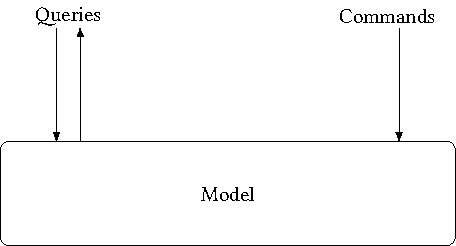
\includegraphics[width=\textwidth]
			{../illustrations/cqs.pdf}
		\caption{
			Command Query Separation (CQS)
		}
		\label{fig:cqs}
	\end{subfigure}
	\quad
	\begin{subfigure}[t]{0.48\textwidth}
	       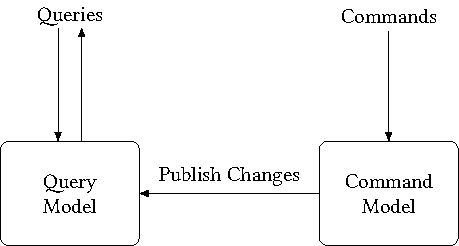
\includegraphics[width=\textwidth]
			{../illustrations/cqrs.pdf}
		\caption{
			Command Query Responsibility Segregation (CQRS)
		}
		\label{fig:cqrs}
	\end{subfigure}
	\caption{Conceptual depiction of both patterns.}
\end{figure}

Command Query Responsibility Segregation is a pattern which was first described 
by Greg Young \cite{Young2013}. In the past, some resources have described it as 
an extension or special case of the Command Query Separation principle, but today 
it is considered a separate pattern with an origin in the CQS principle. 
CQRS states that a different model (i.e. component or object) is used to fulfill 
queries than the model used to fulfill commands (Figure \ref{fig:cqrs}). CQS 
splits responsibilities on the code level, by dividing methods into queries and 
commands; CQRS takes this further and even divides objects into two kinds: 
reading or writing. Young has described this as follows: ``CQRS is simply the 
creation of two objects where there was previously only one'' \cite{Young2010}.

Building an architecture following the CQRS pattern often introduces an 
\emph{eventually consistent} behavior into the system. Since the query and 
command model are separate components, depending on their coupling they might 
not necessarily be in synchronization. 
If they are loosely coupled, the query model does not necessarily contain the 
same data as the command model at every point in time. This characteristic that 
the query model might contain a temporarily inconsistent (i.e. outdated) state, 
which at some point in the future ``eventually'' converges to a consistent state, 
is referred to as eventual consistency.
This eventually consistent behavior becomes especially relevant in distributed 
systems, when the query model(s) are physically separated from the command 
model(s). Brewer's CAP theorem \cite{Brewer1999} postulates that a distributed 
system inevitably has to decide how to handle consistency, since it can only 
ever ensure two of the following three guarantees in case of a network failure:  

\begin{compactenum}
	\item \emph{Consistency}: All participants view the same data.
	\item \emph{Availability}: Each request receives a response.
	\item \emph{Partition Tolerance}: The system continues to operate, 
	even if message loss occurs between arbitrary participants of the
	system. This affects consistency, since participants need to cope
	with the loss of messages. It also affects availability, since each
	participant needs to be able to fulfill requests.
\end{compactenum}

Thus, if a distributed system is built using CQRS as a style of architecture 
and chooses partition tolerance and availability over consistency, the system 
can only provide \emph{eventual} consistency.
Hiding the fact that the system behaves eventually consistent (e.g. by imposing
optimistic assumptions) can be dangerously misleading, since developers and
software components would then operate under false assumptions.
A progressive handling of consistency issues can be seen as a strength of a
distributed ES+CQRS system, since it forces developers to take this very 
consistency behavior -- which is such an integral part of the overall 
architecture -- into account when developing an application. Queries might at 
all times return an outdated result and it is unclear when commands are 
executed. This progressive attitude to issues of large distributed systems has 
spawned a certain kind of attitude and a number of projects in recent years. 
%
The \emph{Reactive Manifesto}~\cite{Boner2014} is a noteworthy document which 
surfaced in 2013. It summarizes key properties behind distributed system design, 
which correspond to event sourcing and CQRS.

\begin{figure}[t]
	\centering
	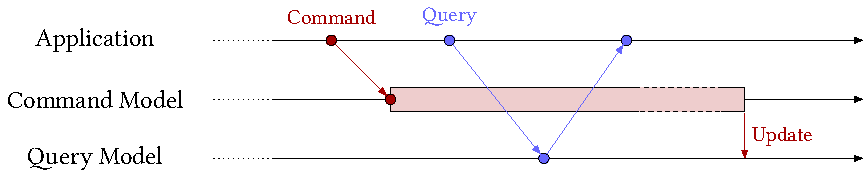
\includegraphics[width=0.8\textwidth]
		{../illustrations/causal-series.pdf}

	\caption{
		In a CQRS architecture, a command and a subsequent
		query do not necessarily possess a causal relationship, since 
		commands are asynchronous and it is unclear when they are
		executed and finished. 
		In the example illustrated above, the query model receives the 
		status update from a finished command after the query has
		already returned. This leads to an eventually consistent
		semantics for queries.
	}
	\label{fig:causal-series}
\end{figure}

A disadvantage of command and query segregation is that it yields a higher 
complexity when building a system and makes it hard to create a causally 
dependent series of commands and events. 
Since commands behave asynchronously and do not return a value, the application 
has no means of knowing when the result of a command is visible.
Thus, a query following a command might return an outdated status.
Subsequent queries, however, will at some point eventually return a consistent 
status. Figure \ref{fig:causal-series} illustrates a typical sequence of commands 
and queries. There are possibilities to circumvent this behavior -- delaying the 
fulfillment of queries until the query model is updated to a certain version 
number for example (as used in conditional requests in 
Eventuate\footnote[1]{\href{https://rbmhtechnology.github.io/eventuate/user\-guide.html\#conditional\-requests}{https://rbmhtechnology.github.io/eventuate/user\-guide.html\#conditional\-requests}}).
%
But it should be noted that these are mitigation techniques which should only 
be used in rare, special cases since they come at the cost of efficiency 
and work against the characteristics of these systems. Instead it is desirable 
for the application to be inherently able to cope with an eventually consistent 
behavior.


\section{Combining ES and CQRS}
\label{sec:es+cqrs}

\begin{figure}[t]
	\centering
	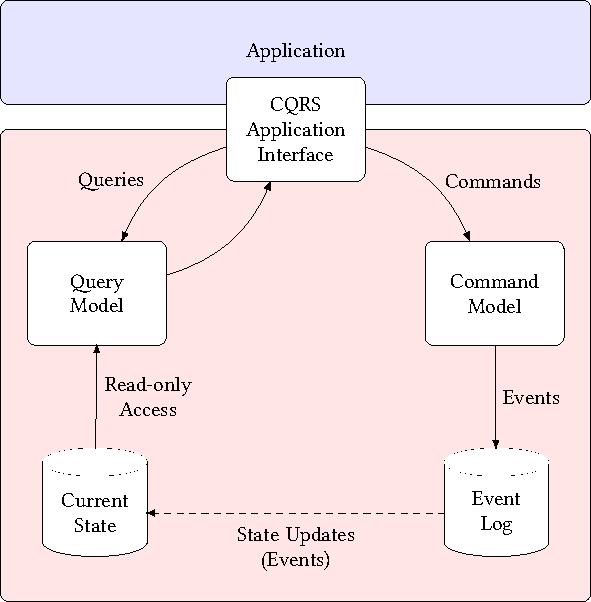
\includegraphics[width=0.5\textwidth]
		{../illustrations/es-cqrs-logic.pdf}

	\caption{
		Architecture of a system which uses event sourcing in 
		combination with CQRS. 
		This illustration is based on a figure from \cite{Erb2014}.}
	\label{fig:escqrs}
\end{figure}

CQRS is a pattern which forms a symbiotic relationship with event sourcing and 
as such is often used in event-sourced architectures.
%
The classification of operations in state-mutating commands and read-only 
queries aligns well with the ideas found in event-sourced systems.
In CQRS, commands represent intentions, which are sent to a command 
processor. There they are processed and yield state changes -- the events.
Events are then appended to the event log and published to query models,
where they eventually update the state as well. Query models fulfill read-only 
requests and can provide a certain view on the data (e.g. a table of accounts 
and their balances). Events are used as the mean to synchronize the models.
%
Thus, commands are then clearly separated from other operations which do not 
result in an append operation to the event log. 
Figure \ref{fig:escqrs} illustrates a typical ES+CQRS architecture: the 
business logic resides in the high level application layer; commands and 
queries hide implementation details of how they are executed. 
Figure \ref{fig:conceptes} depicts a conceptual view with focus on the
internal workings.

The command/query segregation results in characteristics that work well with 
event sourcing. Since events are immutable and are only appended after a 
command has been executed they are the mean to keep data models in 
synchronization. The query models only need to receive new events in order to 
stay consistent with the command model. 
By splitting concerns on an object level, individual optimization of each 
model is supported. 
This is a crucial property for systems with a requirement of scalability,
since the optimization techniques for reads and writes differ.
Segregating the command and query model makes it feasible to scale them 
independently. One technique to optimize for reading operations in a 
distributed system is to replicate the database. These database replicates 
then have to be kept in synchronization, but each of them can then respond 
to requests. A contrasting possibility to optimize for writes, on the other 
hand, is to reduce redundancy (and thus writes) in a database. This can be 
achieved by organizing a single database accordingly, using e.g. normalization 
rules. Further details on the combination of event sourcing and CQRS can be 
found in a work by Hauser \cite{Hauser2014}.

\begin{figure}[h!]
	\centering
	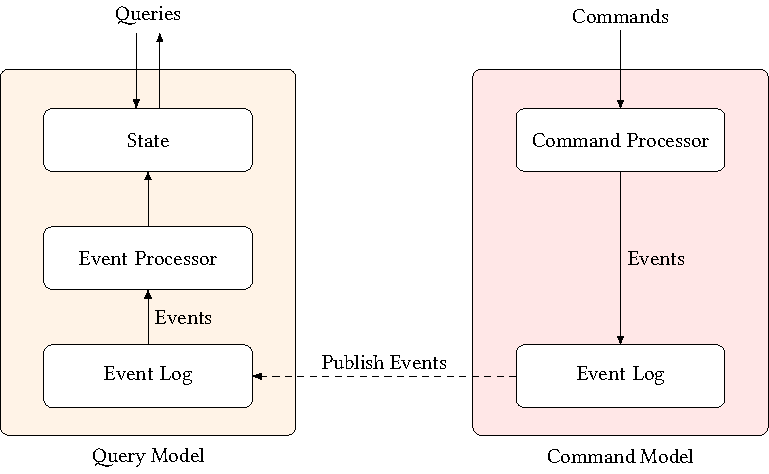
\includegraphics[width=0.67\textwidth]
		{../illustrations/processors.pdf}

	\caption{
		Conceptual view of an event-sourced architecture which takes 
		advantage of the CQRS style.
	}
	\label{fig:conceptes}
\end{figure}

\section{Domain-driven Design (DDD)}
Both, event sourcing and CQRS, are closely related to the idea of domain-driven 
design. The terminology and ideas behind DDD were described by Eric Evans 
\cite{Evans2003} in 2003. At its heart, DDD provides a set of guiding principles 
and building blocks for software development. The core idea here is to put the 
focus of a software project on the domain and the tasks within it. A central part 
when designing a system is the creation of a domain model. Among other components,
this model describes tasks and events of the core domain.
This domain model is created in collaboration with domain experts. In this regard, 
DDD is similar to agile development models, where the collaboration with domain 
experts (or customers) is encouraged as well. 
DDD demands the definition of a common language, the \emph{ubiquitous language}, 
to be used throughout the project. This ubiquitous language is thought to build 
a common view on the domain model amongst team members. Verbs and nouns in the 
language promote a clear understanding of the tasks which need to be fulfilled 
by the system. 
A common language is also thought to prevent misunderstandings and enable anyone 
in a project to talk comprehensibly to any other person in the project, thus 
bringing domain experts and developers together. 

Applying DDD only in this bounded context as well as the usage of high-level 
concepts to abstract from low-level details offer commonalities with the event 
sourcing field.
In an event-sourced system, one usually does not persist all low-level occurring 
events in a system, but rather only relevant domain events in a delimited context. 
DDD is thought to be suited well for systems with complex business rules and a
clearly defined and delimited domain. 
In a simple system, however, DDD may increase complexity to an unnecessary and 
counterproductive level.

The ideas behind event sourcing and CQRS have developed out of DDD. Commands and 
queries in an ES+CQRS system can be modelled using DDD.
This way they have a clear meaning in the domain model and are familiar to 
developers and domain experts. The same holds true for the events which are 
created -- as domain events they fit into the domain model and its logic.
A domain expert describes commands and queries and their internal logic;
an application developer can then access these commands and queries over an
API to implement an application. Since commands and queries abstract from 
domain-specific conditions, working with the system is made easier. 
An application developer does not have to take into account how a command is 
validated or know how it is implemented internally. Complex business logic is 
abstracted through the usage of simplified commands.
